\chapter{Założenia}

\label{ch:zalozenia}

\section{Przykłady systemów akwizycji danych}

Na rynku jest dostępna szeroka gama systemów akwizycji danych. Większość dostępnych rozwiązań to układy do profesjonalnych zastosowań laboratoryjnych. Często urządzenia te pracują tylko pod określonym oprogramowaniem co zwiększa koszty. Powoduje to, że brakuje urządzeń, które posiadałyby podstawową funkcjonalność systemu akwizycji danych za cenę mniejszą niż 500zł. 

\subsection{System akwizycji danych NI USB6008}

Przykładem jest system akwizycji danych National Instruments USB6008. Urządzenie posiada 8 analogowych wejść i obsługuje interfejs USB. Zawiera 12-bitowy przetwornik analogowo-cyfrowy próbkujący z częstotliwością 10kS/s.\cite{NI_6008} Urządzenie kosztuje około 1000zł w celu wykonania pomiarów potrzebujemy komputera z zainstalowanym oprogramowaniem producenta, co powoduje generowanie dodatkowych kosztów.

\begin{figure}[h]
	\centering
		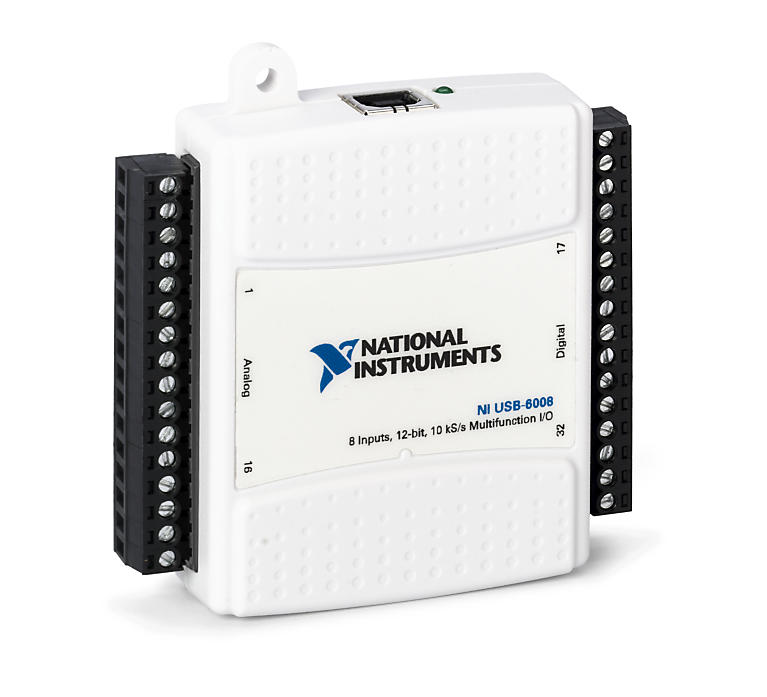
\includegraphics[width=10cm]{daq_ni_usb6008}
	\caption{National Instruments USB6008} 
	\label{fig:uxtouch}
\end{figure}

\subsection{Oscyloskop cyfrowy Digilent Analog Discovery 2}

Kolejnym przykładem systemu akwizycji danych jest przystawka do komputera osobistego  Digilent Analog Discovery 2. Urządzenie po podłączeniu do komputera PC oraz doprowadzeniu badanych sygnałów do jego wejść umożliwia wykonywanie pomiarów. Posiada następujące parametry techniczne\cite{AnalogDiscoveryDoc}

\begin{itemize}
\item 16-kanałowy analizator logiczny (14-bit, 100MS/s, +-5V) 
\item 2-kanałowy oscyloskop cyfrowy (14-bitowy, 100MS/s, +-25V) 
\item wzmacniacz audio-stereo, 
\item interfejsy SPI, I2C, UART, USB
\item zasilanie 5V
\end{itemize}

\begin{figure}[h]
	\centering
		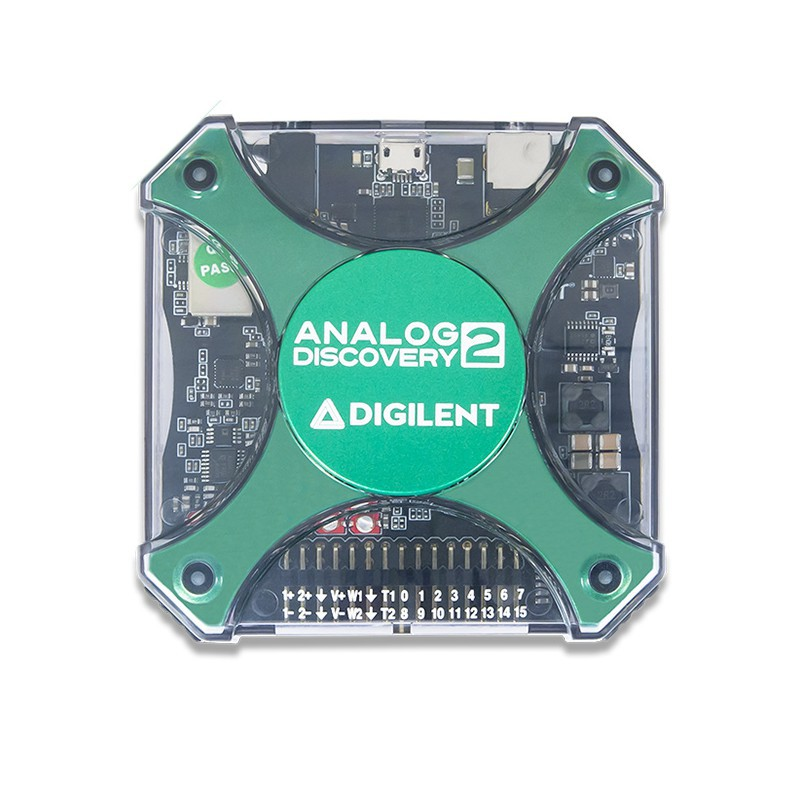
\includegraphics[width=10cm]{analog_discovery2}
	\caption{Digilent Analog Discovery 2} 
	\label{fig:uxtouch}
\end{figure}


Cena urządzenia jest zbliżona do poprzedniego przykładu (ok. 1000-1400zł), jednak oprogramowanie, pozwalające na pracę z przystawką jest darmowe, co znacząco obniża koszt całego systemu. Nie mniej jednak sama przystawka Digilent Analog Discovery 2 nie tworzy w pełni funkcjonalnego systemu akwizycji danych. Do poprawnego działania systemu potrzebny jest komputer osobisty z zainstalowanym dedykowanym oprogramowaniem.

Powyższe urządzenia nie posiadają interfejsu sieciowego. Zapewniają jedynie możliwość akwizycji danych na podłączonym przez port USB komputerze.

\section{Cechy systemu}
System powinien udostępniać możliwość obsługi sygnałów zarówno cyfrowych jak i analogowych. Ze względu na brak przetwornika analogowo-cyfrowego na płytce Raspberry Pi, konieczne jest użycie zewnętrznego układu.
Raspberry Pi może działać pod systemem operacyjnym Linux, który nie jest systemem czasu rzeczywistego, co powoduje, że w domyślnej konfiguracji systemu nie da się zagwarantować stałego odstępu czasowego pomiędzy odbieraniem próbek kolejnych z przetwornika. W celu wydajnego przetwarzania sygnałów większej częstotliwości dodano moduł do jądra systemu, zawierający implementację licznika wysokiej rozdzielczości, co powoduje zmniejszenie wahań częstotliwości próbkowania w trakcie pomiarów oraz pozwala na zachowanie momentu otrzymania próbki z dużą dokładnością.

\subsection{Informacja o czasie pomiaru}

Raspberry Pi jest komputerem zoptymalizowanym pod względem kosztów, co sprawia, że jest pozbawiony podzespołów, które są zbyt drogie. Jednym z takich układów jest układ RTC (z ang. Real Time Clock - zegar czasu rzeczywistego) Układ ten jest zasilany z baterii niezależnie od komputera i zapewnia przechowywanie czasu rzeczywistego po odłączeniu zasilania komputera. System akwizycji danych powinien zapewniać w miarę możliwości technicznych jak najdokładniejszą informację o czasie zebrania próbki danych.
Raspberry Pi za pomocą protokołu NTP (z ang. Network Time Protocol - Sieciowy Protokół Czasu) jest w stanie synchronizować czas w systemie do wybranego w konfiguracji protokołu serwera. Konfigurację Korzystając z odpowiednich serwerów, NTP jest w stanie dostosować czas systemu klienta, uwzględniając opóźnienia w transmisji danych.

Wykorzystanie własnego sterownika do pomiaru napięcia przetwornika analogowo-cyfrowego pozwala na zebranie znacznika czasu z dokładnością do pojedynczych nanosekund.   

\section{Struktura systemu}

System składa się z platformy Raspberry Pi używanej jako komputer główny oraz dołączanej płytki pomiarowej umożliwiającej podłączenie czujników z możliwością łatwego doprowadzenia zasilania do wszystkich urządzeń. Platforma Raspberry Pi zapewnia w systemie kontrolę pomiarów i pozwala na wizualizację oraz udostępnianie otrzymanych wyników. 


\begin{figure}[h]
	\centering
		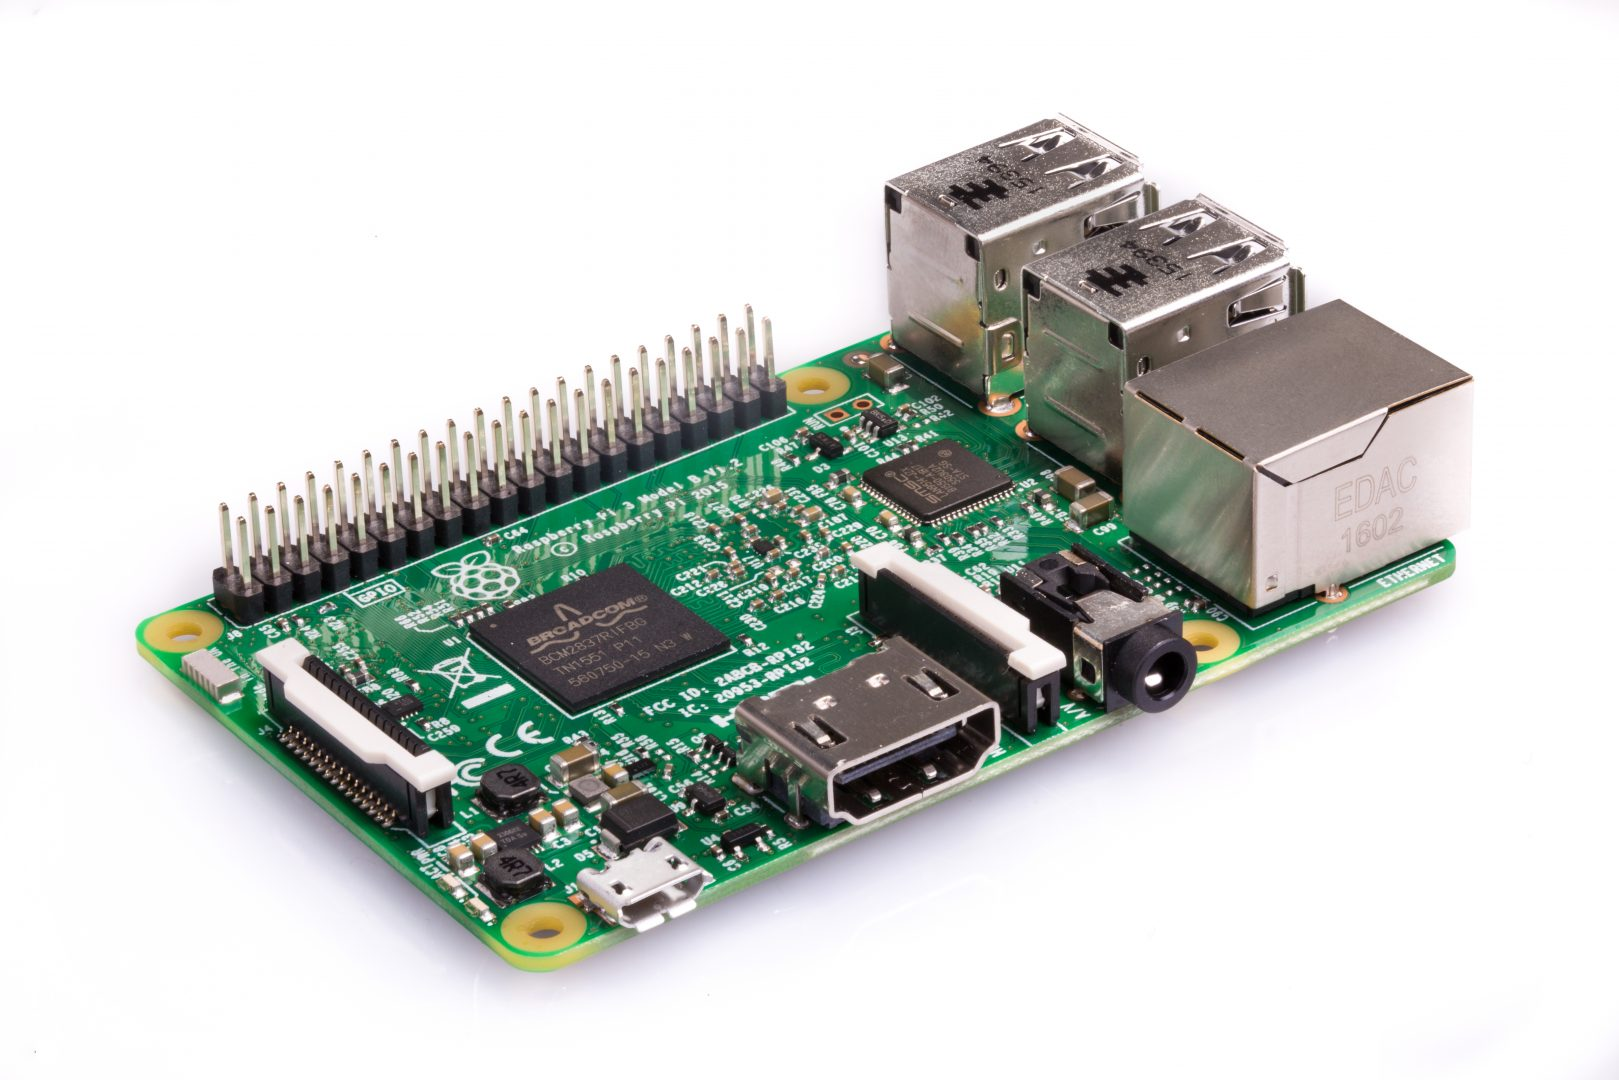
\includegraphics[width=10cm]{rpi}
	\caption{Raspberry Pi 3 Model B} 
	\label{pic:RPi}
\end{figure}

\subsection{Platforma Raspberry Pi}

Raspberry Pi to jednopłytkowa platforma stworzona przez Raspberry Pi Foundation. Pierwsza wersja minikomputera powstała w roku 2012 i była oparta o układ firmy Broadcom BCM2835 SoC (z ang. System on Chip - System wbudowany) oraz procesor graficzny Broadcom VideoCore IV. Głównymi zaletami platformy były niska cena w stosunku do możliwości. 
Platforma Raspberry Pi w wersji 3 posiada liczne złącza m.in.: HDMI, Ethernet, 4 porty USB 2.0, wyjście 3,5mm jack, złącze kart microSD oraz 40-pinowe złącze GPIO. W tabeli poniżej przedstawiono specyfikacje wersji płytki użytej w projekcie - Raspberry Pi 3 Mdel B:

\begin{table}[t]
\label{tabRpi}
\centering
\begin{tabular}{|l|l|l|}
  \hline 
  Nazwa układu SoC & Broadcom BCM2837 \\
  \hline
  Procesor CPU & 1,2 GHz quad-core ARM Cortex-A53 (64-bit) \\
  \hline
 Procesor graficzny GPU & Broadcom VideoCore IV \\ 
  \hline 
  Pamięć RAM  & 1 GB LPDDR2 (900 MHz) \\
  \hline
 Napięcie zasilania & 5 V, złącze MicroUSB lub GPIO\\
  \hline
 Połączenia sieciowe & 10/100 Ethernet, Wi-Fi (2,4 GHz 802.11n) \\
  \hline
 Nośnik danych  & złącze kart MicroSD \\
 \hline
 
\end{tabular}
\caption{Parametry techniczne platformy Raspberry Pi 3 Model B 
\cite{rpispecs}
} 
\end{table}

\begin{figure}[h]
	\centering
		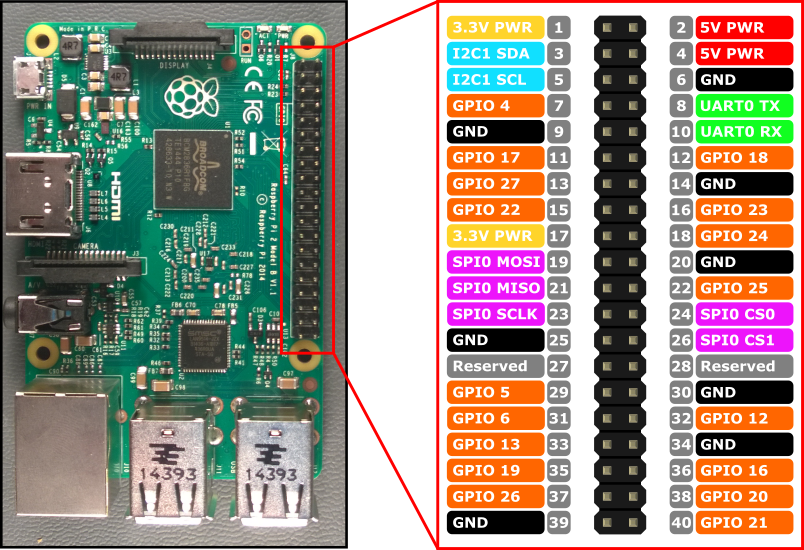
\includegraphics[width=12cm]{rpipinout}
	\caption{Rozkład pinów GPIO na płytce Raspberry Pi} 
	\label{pic:rpipinout}
\end{figure}



\subsection{Płytka pomiarowa}

Płytka pomiarowa, stanowiąca rozszerzenie do Raspberry Pi, miała umożliwiać podłączenie czujników do minikomputera oraz doprowadzenie do nich zasilania i została wykonana na potrzeby pracy dyplomowej. 
Zastosowanie przetwornika analogowo-cyfrowego pozwala na zbieranie danych z czujników analogowych. Czujniki cyfrowe podłączone przez magistralę SPI lub I2C powinny być wydajnie obsługiwane przez system.

\subsection{Założenia oprogramowania}

Oprogramowanie powinno umożliwiać przeprowadzenie wydajnej akwizycji, bez utraty danych.
Niezbędne jest skorzystanie z odpowiednich bibliotek i funkcji udostępnianych przez jądro systemu Linux. Aplikacje użytkownika powinny zapisywać dane do pliku w formacie umożliwiającym późniejsze przetworzenie przez aplikację obsługującą protokół sieciowy MQTT i aplikację umożliwiającą wyświetlanie danych i ustawienie konfiguracji parametrów pomiaru uruchamianą przez użytkownika w przeglądarce internetowej. Aplikacja udostępnia interfejs pozwalający na zdalne uruchomienie programów obsługujących Oprogramowanie powinno posiadać cechy przenośności tak, aby mogło działać na innych systemach wbudowanych z systemem operacyjnym Linux.

